\section{Introduction}

\subsection{General steps to manufacture quantum dots}

The steps for manufacture are described below:\\

\begin{enumerate}[noitemsep]
\item Cleaving
\item Cleaning
\item Resist spinning
\item Photolithography (mesa pattern)
\item Resist developing
\item Mesa etching
\item Resist removal (5\,min sonication in NMP, rince with IPA)
\item Resist spinning (including cleaning on chuck)
\item Photolithography (ohmics pattern)
\item Resist developing
\item Plasma ash
\item Metal deposition (ohmics)
\item Lift-off
\item Annealing
\item Resist spinning
\item Electron Beam Lithography (fine gates)
\item Plasma ash
\item Metal deposition (fine gates)
\item Lift-off
\item Cleaning
\item Resist spinning
\item Photolithography (large gates)
\item Resist developing
\item Plasma ash
\item Metal deposition
\item Lift-off
\item Imaging
\end{enumerate}

\newpage

\subsection{Alignments DD V1}

\begin{figure} [h] \centering
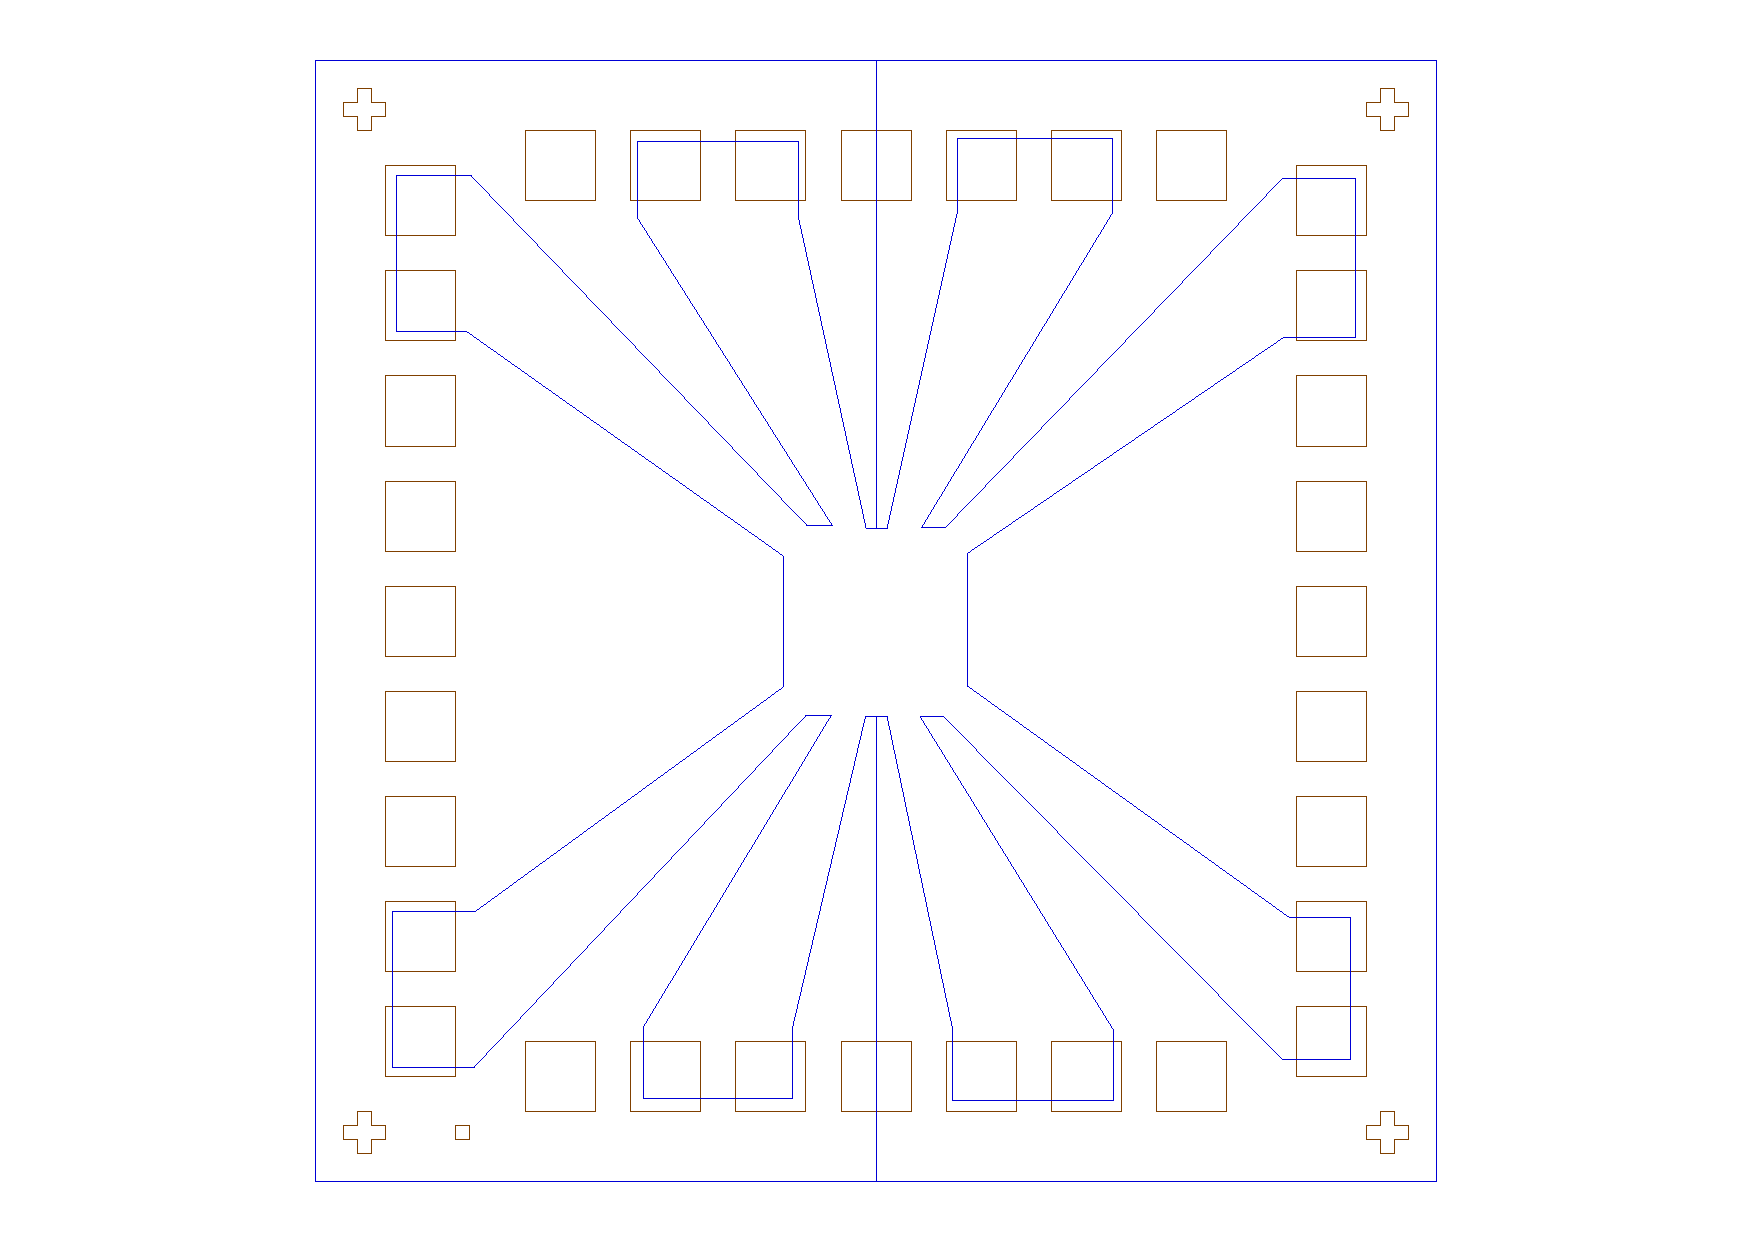
\includegraphics[scale=0.3]{fig/align1.pdf}
\caption{Alignment of the ohmics patern with the mesa patern.} \label{align1}
\end{figure}

\begin{figure} [h] \centering
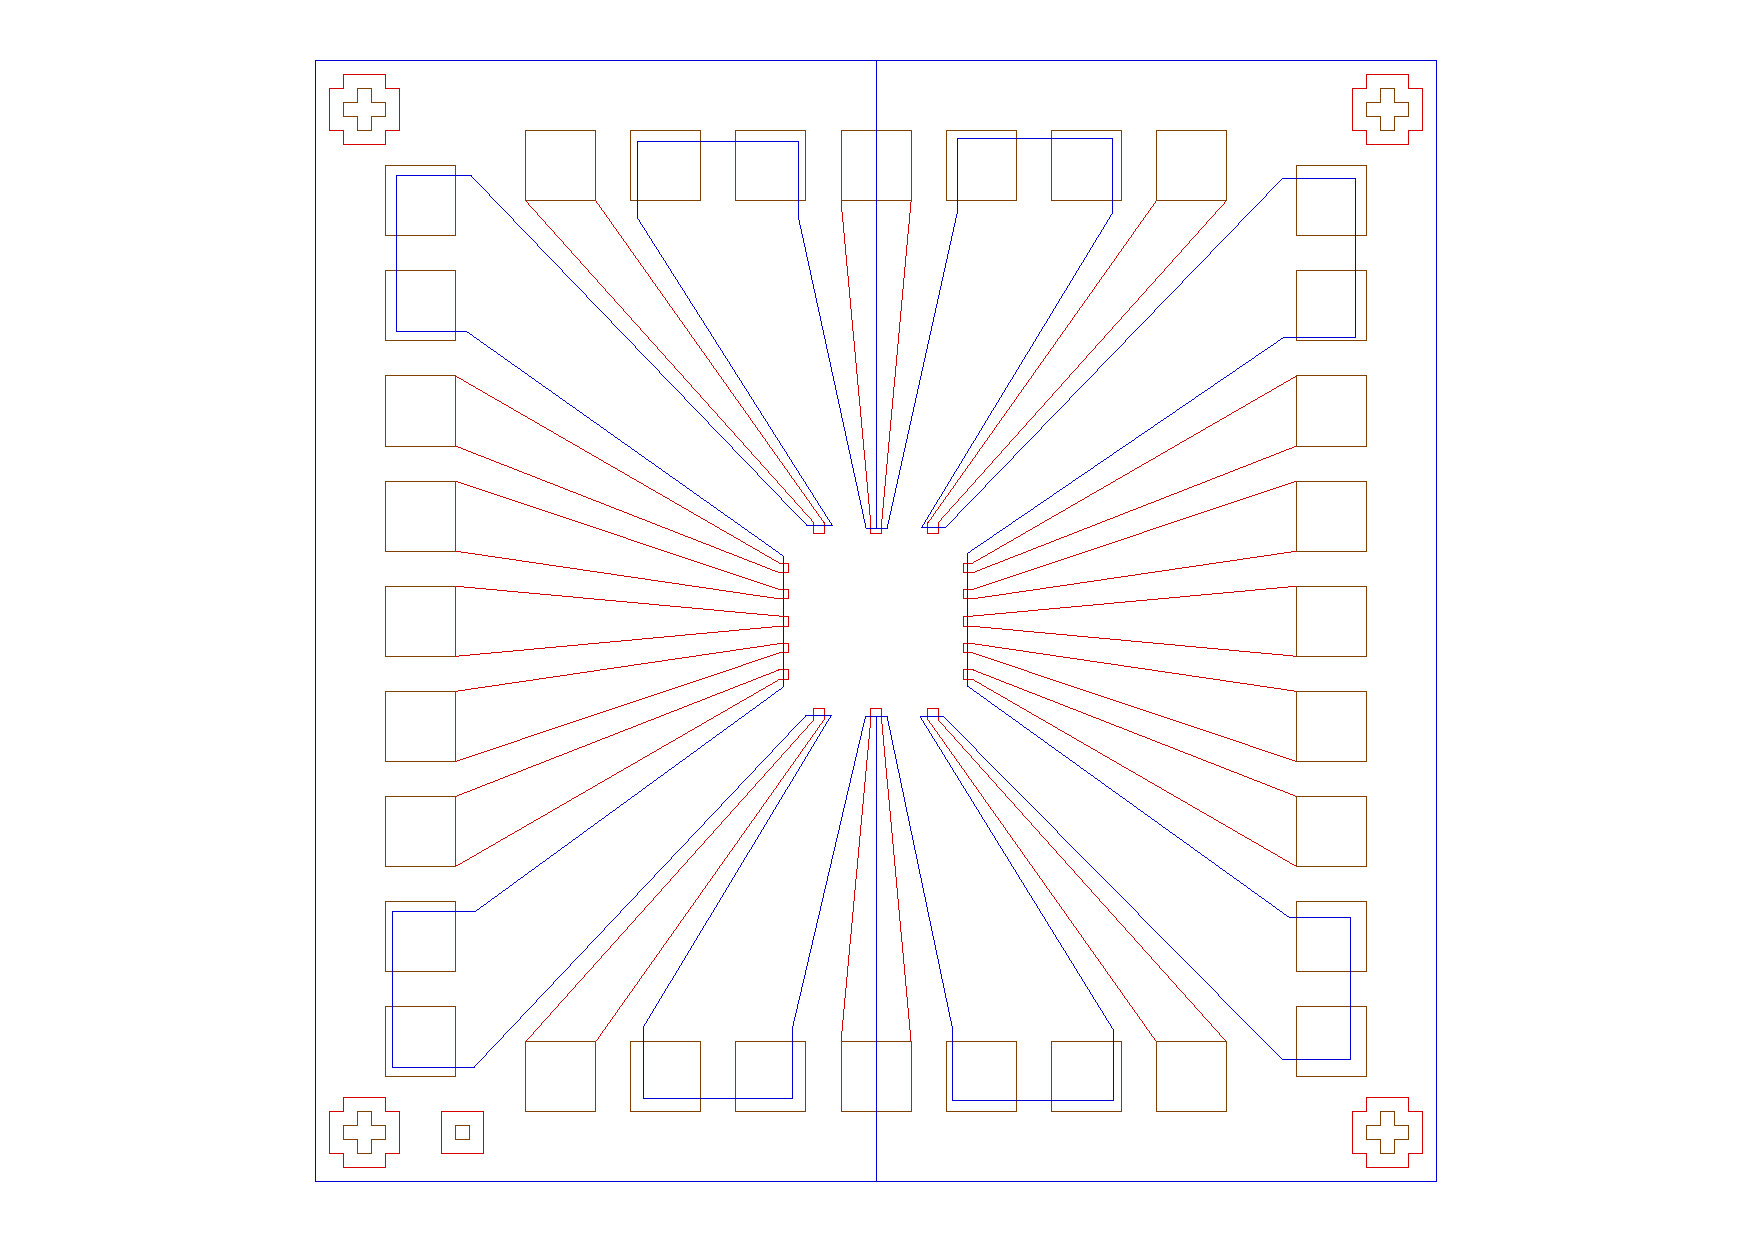
\includegraphics[scale=0.3]{fig/align2.pdf}
\caption{Alignment of the contacts with the ohmics and mesa paterns.} \label{align2}
\end{figure}

\newpage

\subsection{Alignments DD V2}

\begin{figure} [h] \centering
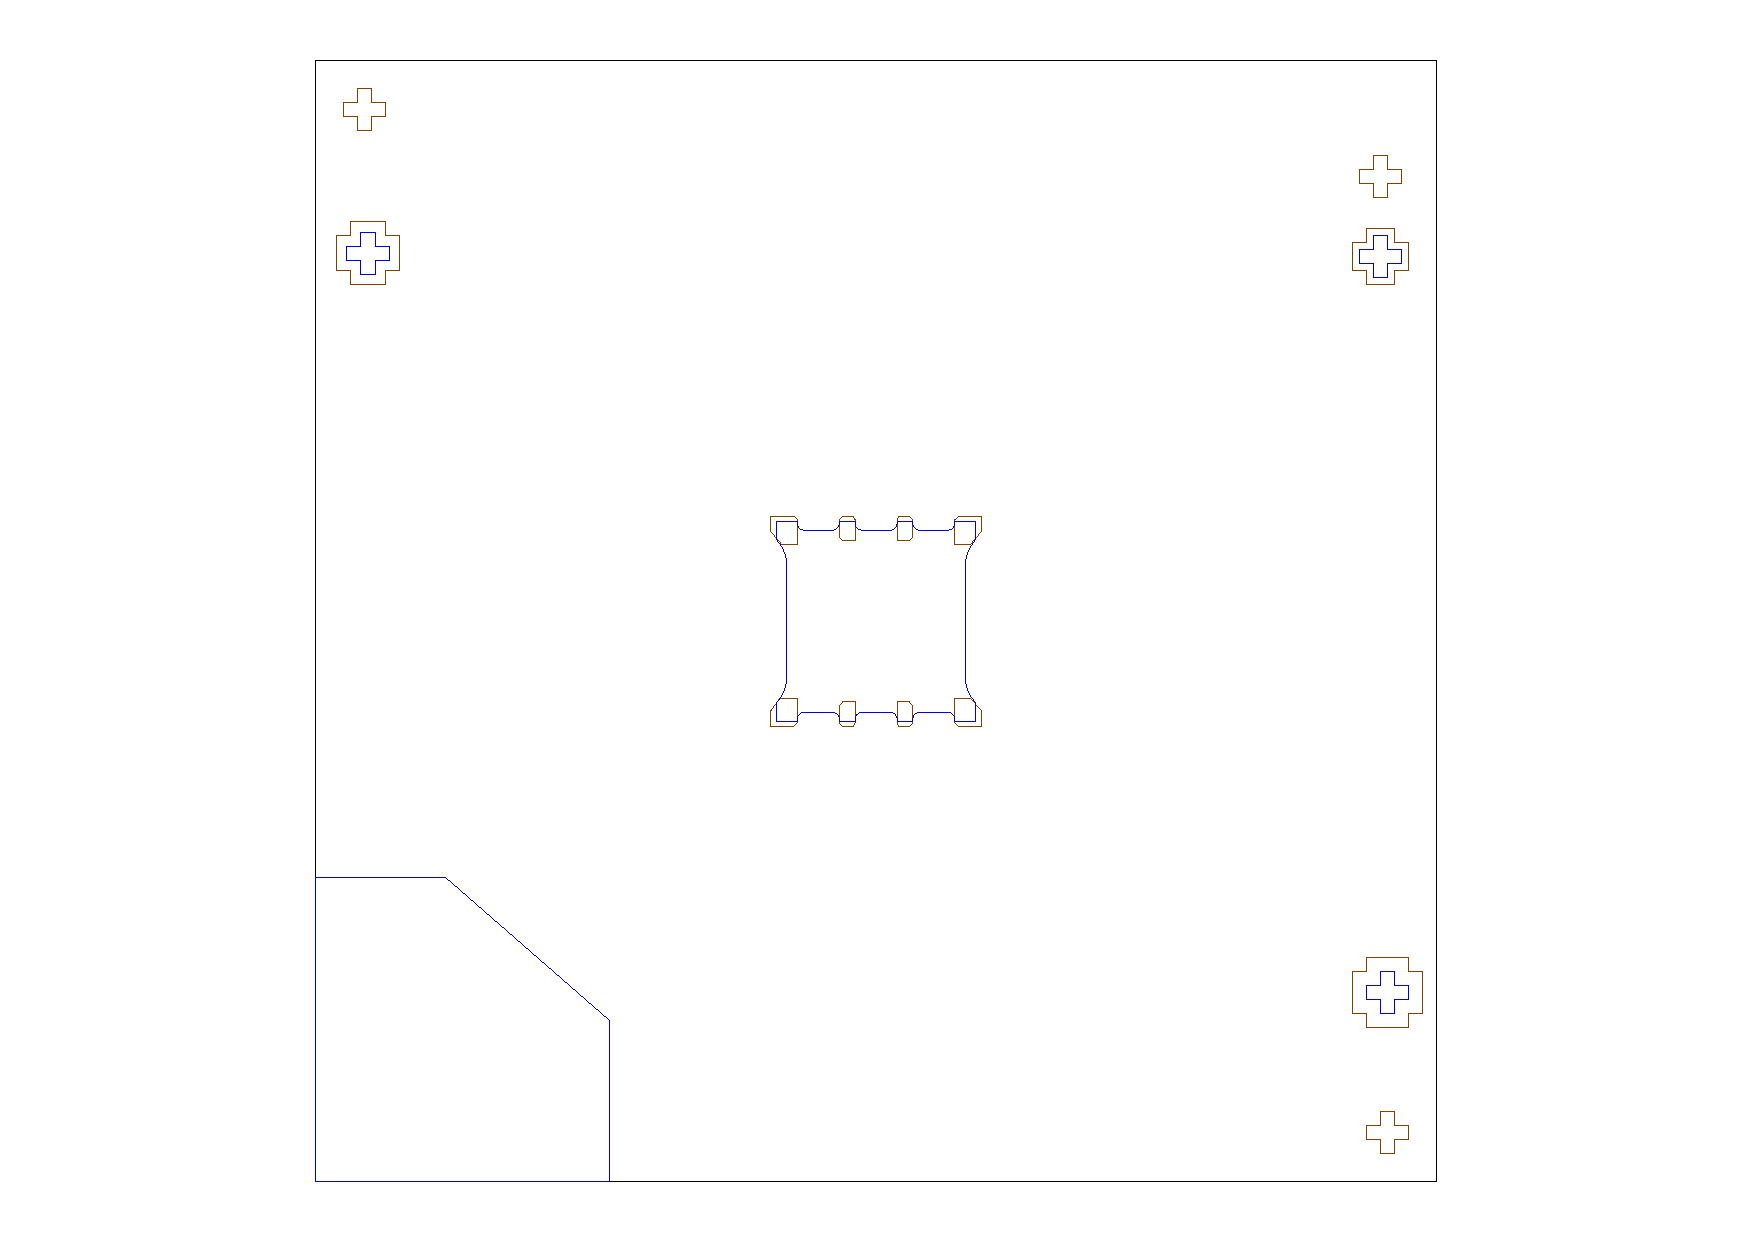
\includegraphics[scale=0.3]{fig/align1_1.pdf}
\caption{Alignment of the ohmics patern with the mesa patern.} \label{align1}
\end{figure}

\begin{figure} [h] \centering
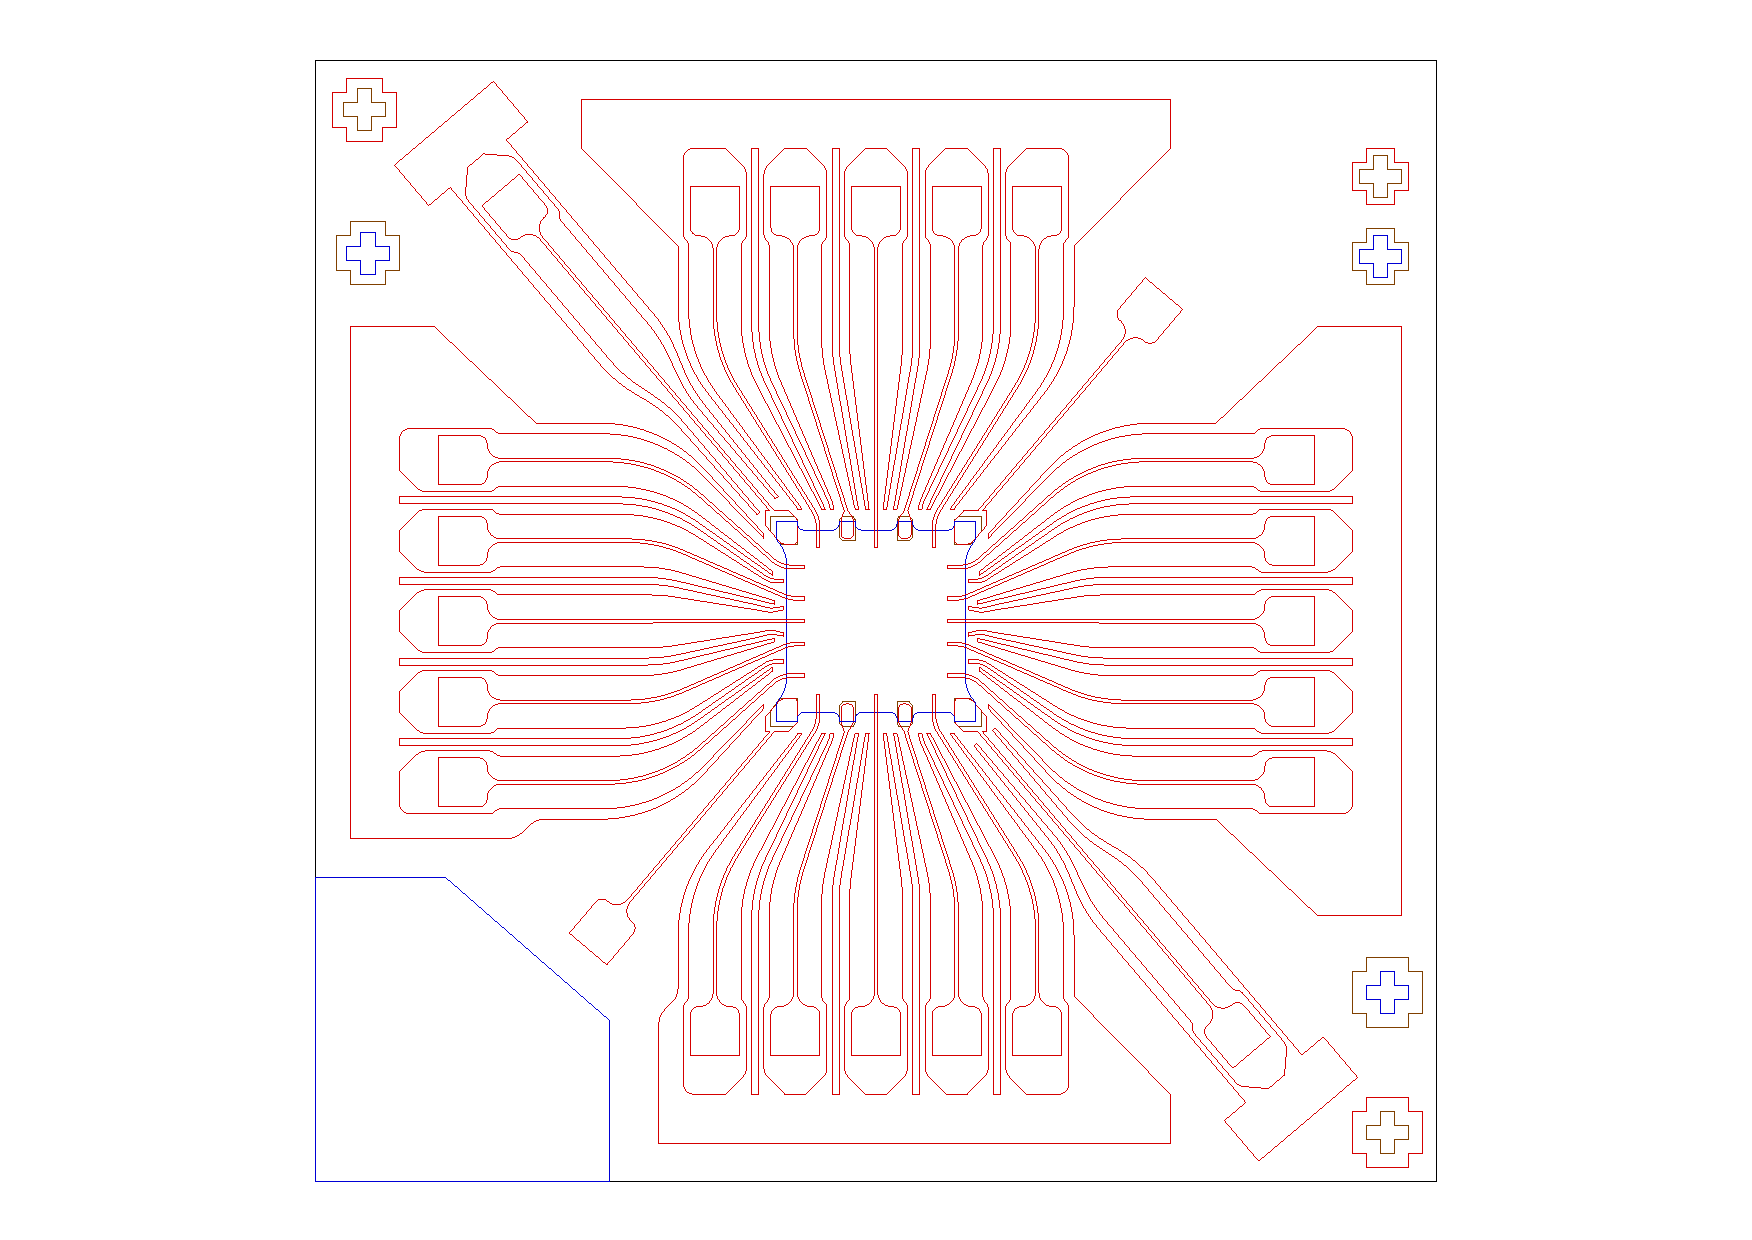
\includegraphics[scale=0.3]{fig/align2_1.pdf}
\caption{Alignment of the contacts with the ohmics and mesa paterns.} \label{align2}
\end{figure}



\newpage

\subsection{Dressing}
\begin{itemize}
\item mask
\item hair nest
\item suit
\item shoes (!on other side of bench!)
\item gloves
\item glasses
\end{itemize}

The clean room begin just after the bench in front of the door. DON'T SIT ON THE BENCH.

Note: If you have your own cleanroom gown, it can be picked up in the grey area of the Upper East labs.
Tick your name off on the spreadsheet and grab a head cover, overalls and boots from the lockers corresponding
to your size.

\subsection{Misc}

\begin{itemize}
\item Tools in lunch box
\item Clean everything you need/use
\item Write up EVERYTHING, make protocols
\item To quickly remove the water in beakers, spray IPA and blow dry
\item If the chip is flipped: clean and re-spin
\item Inside fume hoods, always manipulate beakers and
chip on wipes (to avoid losing the chip in holes).
\item If a solvent container is empty, open it and let it out gas inside
the cupboard on the left hand side.
\item If the solvent waste is full, take an empty solvent container,
pour the solvent waste in it and put it in the bottom left hand
side shelve, on the left of the cupboard. Put a provided sticker
on it.
\end{itemize}

\newpage

